\documentclass{beamer}
\usepackage{tikz,amsmath,amssymb,hyperref,graphicx,stackrel,animate}
\usetikzlibrary{positioning,shadows,arrows,shapes,calc}
\newcommand{\argmax}{\operatornamewithlimits{argmax}}
\newcommand{\argmin}{\operatornamewithlimits{argmin}}
\mode<presentation>{\usetheme{Frankfurt}}
\AtBeginSection[]
{
  \begin{frame}<beamer>
    \frametitle{Outline}
    \tableofcontents[currentsection,currentsubsection]
  \end{frame}
}
\title{Lecture 3: Noise}
\author{Mark Hasegawa-Johnson}
\date{ECE 417: Multimedia Signal Processing, Fall 2020}  
\begin{document}

% Title
\begin{frame}
  \maketitle
\end{frame}

% Title
\begin{frame}
  \tableofcontents
\end{frame}

%%%%%%%%%%%%%%%%%%%%%%%%%%%%%%%%%%%%%%%%%%%%
\section[Motivation]{Motivation: Noisy Telephones}
\setcounter{subsection}{1}

\begin{frame}
  \frametitle{Noisy Telephones}
  \begin{itemize}
  \item In the 1920s, Harvey Fletcher had a problem.
  \item Telephones were noisy (very noisy).
  \item Sometimes, people could hear the speech.  Sometimes not.
  \item Fletcher needed to figure out why people could or couldn't hear the
    speech, and what Western Electric could do about  it.
  \end{itemize}
\end{frame}

\begin{frame}
  \frametitle{Tone-in-Noise Masking Experiments}

  He began playing people pure tones mixed with noise, and asking
  people ``do you hear a tone''?  If 50\% of samples actually
  contained a tone, and if the listener was right 75\% of the time, he
  considered the tone ``audible.''
  \centerline{\includegraphics[height=2in]{exp/tone_white_waveform.png}}
\end{frame}

\begin{frame}
  \frametitle{Tone-in-Noise Masking Experiments}

  People's ears are astoundingly good.  This tone is inaudible in this
  noise.  But if the tone was only $2\times$ greater amplitude, it
  would be audible.
  \centerline{\includegraphics[height=2in]{exp/tone_white_waveform.png}}
\end{frame}

\begin{frame}
  \frametitle{Tone-in-Noise Masking Experiments}

  Even more astounding: the same tone, in a very slightly different noise,
  is perfectly audible, to every listener.
  \centerline{\includegraphics[height=2in]{exp/tone_bandstop_waveform.png}}
\end{frame}

\begin{frame}
  \frametitle{What's going on (why can listeners hear the difference?)}
  \centerline{\includegraphics[height=1.5in]{exp/tone_white_waveform.png}}
  \centerline{\includegraphics[height=1.5in]{exp/tone_bandstop_waveform.png}}
\end{frame}

%%%%%%%%%%%%%%%%%%%%%%%%%%%%%%%%%%%%%%%%%%%%
\section[Filters]{Auditory Filters}
\setcounter{subsection}{1}

\begin{frame}
  \frametitle{Review: Discrete Fourier Transform}

  Remember the discrete Fourier transform (DFT):
  \[
  X[k] = \sum_{n=0}^{N-1} x[n]e^{-j\left(\frac{2\pi  kn}{N}\right)},~~~~~
  x[n]=\frac{1}{N}\sum_{k=0}^{N-1} X[k]e^{j\left(\frac{2\pi  kn}{N}\right)}
  \]
  This is useful because, unlike $X(\omega)$, we can actually compute
  it on a computer (it's discrete in both time and frequency).  If
  $x[n]$ is finite length (nonzero only for $0\le n\le N-1$), then
  \[
  X[k] = X\left(\omega=\frac{2\pi k}{N}\right)
  \]
  We sometimes write this as $X[k]=X(\omega_k)$, where, obviously, $\omega_k=\frac{2\pi k}{N}$.
\end{frame}
  
\begin{frame}
  \frametitle{What's going on (why can listeners hear the difference?)}
  \centerline{\includegraphics[height=1.5in]{exp/tone_white_waveform.png}}
  \centerline{\includegraphics[height=1.5in]{exp/tone_bandstop_waveform.png}}
\end{frame}

\begin{frame}
  \frametitle{Fourier to the Rescue}

  Here's the DFT power spectrum ($|X[k]|^2$) of the tone, the white
  noise, and the combination.
  \centerline{\includegraphics[height=2in]{exp/tone_white_powerspectrum.png}}
\end{frame}

\begin{frame}
  \frametitle{Bandstop Noise}

  The ``bandstop'' noise is called ``bandstop'' because I arbitrarily set
  its power to zero in a small frequency band centered at 1kHz.  Here is the
  power spectrum.  Notice that, when the tone is added to the noise signal, 
  the little bit of extra power makes a noticeable (audible) change, because
  there is no other power at that particular frequency.
  \centerline{\includegraphics[height=2in]{exp/tone_bandstop_powerspectrum.png}}
\end{frame}

\begin{frame}
  \frametitle{Fletcher's Model of Masking}

  Fletcher proposed the following model of hearing in noise:
  \begin{enumerate}
  \item The human ear pre-processes  the audio using a bank of bandpass filters.
  \item The power of the noise signal, in the $k^{\textrm{th}}$
    bandpass filter, is $N_k$.
  \item The power of the noise+tone is $N_k+T_k$.
  \item If there is {\bf\em any} band, $k$, in which
    $\frac{N_k+T_k}{N_k}>\mbox{threshold}$, then the tone is audible.
    Otherwise, not.
  \end{enumerate}
\end{frame}

\begin{frame}
  \frametitle{Von Bekesy and the Basilar Membrane}

  \begin{itemize}
  \item In 1928, Georg von B{\'{e}}k{\'{e}}sy found Fletcher's auditory
    filters.
  \item Surprise: they are {\bf\em mechanical}.
  \item The inner ear contains a long (3cm), thin (1mm), tightly
    stretched membrane (the basilar membrane).  Like a steel drum, it
    is tuned to different frequencies at different places: the outer
    end is tuned to high frequencies, the inner end to low
    frequencies.
  \item About 30,000 nerve cells lead from the basilar membrane to the
    brain stem.  Each one sends a signal if its part of the basilar
    membrane vibrates.
  \end{itemize}
\end{frame}

\begin{frame}
  \centerline{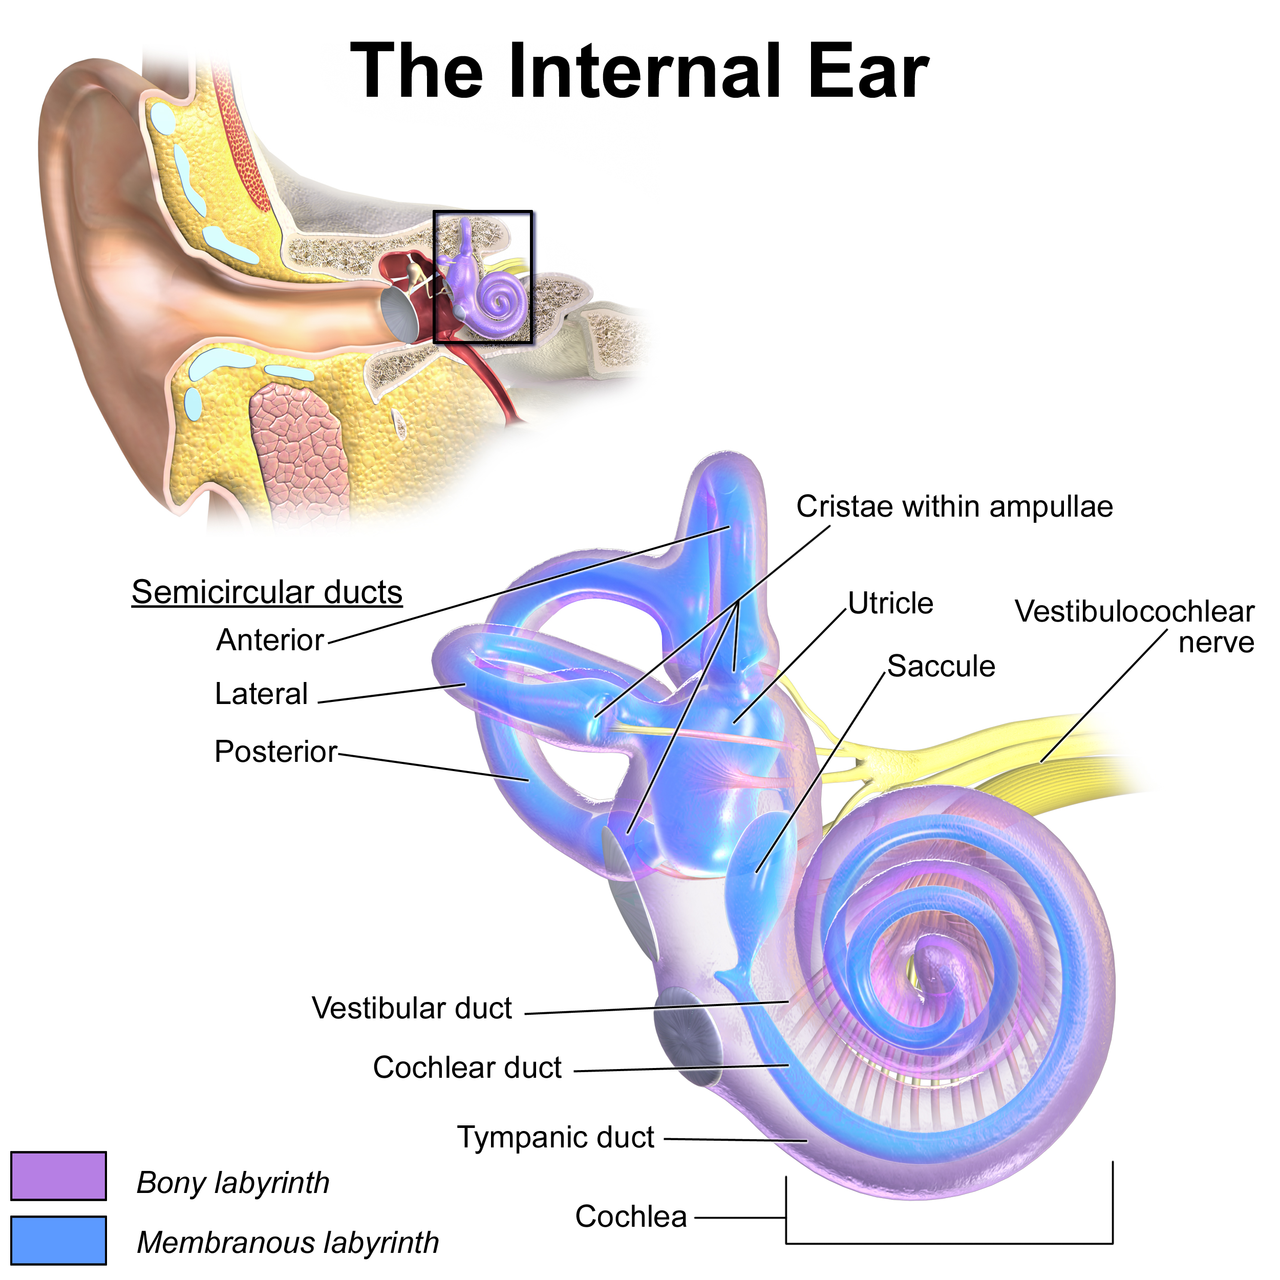
\includegraphics[height=3in]{Blausen_0329_EarAnatomy_InternalEar.png}}
  \begin{tiny}
    Blausen.com staff (2014). ``Medical gallery of Blausen Medical
    2014.'' WikiJournal of Medicine 1
    (2). DOI:10.15347/wjm/2014.010. ISSN 2002-4436.
  \end{tiny}
\end{frame}

\begin{frame}
  \centerline{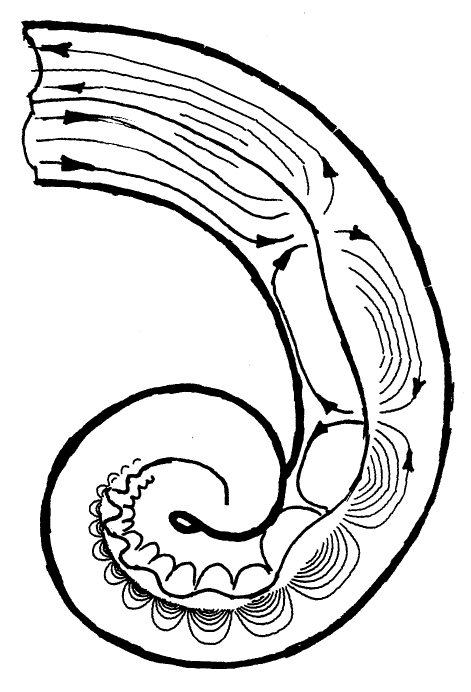
\includegraphics[height=3in]{Cochlea_Traveling_Wave.png}}
  \begin{tiny}
    Dick Lyon, public domain image, 2007.
    \url{https://en.wikipedia.org/wiki/File:Cochlea_Traveling_Wave.png}
  \end{tiny}
\end{frame}

\begin{frame}
  \frametitle{Frequency responses of the auditory filters}

  Here are the squared magnitude frequency responses ($|H(\omega)|^2$)
  of 26 of the 30000 auditory filters. I plotted these using the
  parametric model published by Patterson in 1974:
  \centerline{\includegraphics[height=2in]{exp/gammatone_filterbank.png}}
\end{frame}
     
\begin{frame}
  \frametitle{Filtered white noise}

  An acoustic white  noise signal (top), filtered through a spot on the
  basilar membrane with a particular impulse response (middle), might result in
  narrowband-noise  vibration of the basilar membrane (bottom).
  \centerline{\includegraphics[height=2in]{exp/gtfiltered_white_waveform.png}}
\end{frame}
     
\begin{frame}
  \frametitle{Filtered white noise}

  An acoustic white  noise signal (top), filtered through a spot on the
  basilar membrane with a particular impulse response (middle), might result in
  narrowband-noise  vibration of the basilar membrane (bottom).
  \centerline{\includegraphics[height=2in]{exp/gtfiltered_white_powerspectrum.png}}
\end{frame}
     
\begin{frame}
  \frametitle{Tone + Noise: Waveform}

  If there is a tone embedded in the noise, then even after filtering, it's
  very hard to see that the tone is there\ldots
  
  \centerline{\includegraphics[height=2in]{exp/gtfiltered_tone_white_waveform.png}}
\end{frame}
     
\begin{frame}
  \frametitle{Filtered white noise}

  But, Fourier comes to the rescue!  In the power spectrum, it is
  almost possible, now, to see that the tone is present in the white noise masker.
  
  \centerline{\includegraphics[height=2in]{exp/gtfiltered_tone_white_powerspectrum.png}}
\end{frame}
     
\begin{frame}
  \frametitle{Filtered bandstop noise}

  If the masker is bandstop noise, instead of white noise, the spectrum
  after filtering looks very different\ldots
  
  \centerline{\includegraphics[height=2in]{exp/gtfiltered_bandstop_powerspectrum.png}}
\end{frame}
     
\begin{frame}
  \frametitle{Filtered tone + bandstop noise}

  \ldots and the tone+noise looks very, very different from the noise by itself.
  \centerline{\includegraphics[height=2in]{exp/gtfiltered_tone_bandstop_powerspectrum.png}}
  \centerline{\huge This is why the tone is audible!}
\end{frame}

\begin{frame}
  \frametitle{What an excellent model!  Why should  I believe it?}

  Let's spend the rest of today's lecture talking about:
  \begin{itemize}
  \item What is a power spectrum?
  \item What is noise?
  \item What is autocorrelation?
  \end{itemize}
  Then, next lecture, we will find out what happens to noise when it gets
  filtered by an auditory filter.
\end{frame}

%%%%%%%%%%%%%%%%%%%%%%%%%%%%%%%%%%%%%%%%%%%%
\section[Power]{Power Spectrum}
\setcounter{subsection}{1}

\begin{frame}
  \frametitle{What is power?}

  \begin{itemize}
    \item Power (Watts=Joules/second) is usually the time-domain
      average of amplitude squared.
    \item Example: electrical power $P=R\overline{i^2(t)} = \overline{v^2(t)}/R$
    \item Example: acoustic power $P=\langle z_0 \overline{u^2(t)}\rangle = \overline{p^2(t)}/z_0$
    \item Example: mechanical power (friction) $P= \mu\overline{v^2(t)} = \overline{f^2(t)}/\mu$
  \end{itemize}
  where, by $\overline{x^2(t)}$, I mean the time-domain average of $x^2(t)$.
\end{frame}

\begin{frame}
  \frametitle{What is power?}

  In signal processing, we abstract away from the particular problem,
  and define instantaneous power as just
  \[
  P = \overline{x^2(t)}
  \]
  or, in  discrete time,
  \[
  P = \overline{x^2[n]}
  \]
\end{frame}
  
\begin{frame}
  \frametitle{Parseval's Theorem for Energy}

  Parseval's theorem tells us that the energy of a signal is the same
  in both the time domain and frequency domain.  Here's Parseval's
  theorem for the DTFT:
  \[
  \sum_{n=-\infty}^{\infty}x^2[n] = \frac{1}{2\pi}\int_{-\pi}^{\pi}\left|X(\omega)\right|^2d\omega
  \]
  \ldots and here it is for the DFT:
  \[
  \sum_{n=0}^{N-1}x^2[n] = \frac{1}{N}\sum_{k=0}^{N-1}\left|X[k]\right|^2
  \]  
\end{frame}

\begin{frame}
  \frametitle{Parseval's Theorem}

  Notice that the white noise spectrum (middle window, here) has an energy of exactly
  \[
  \frac{1}{N}\sum_{k=0}^{N-1}\left|X[k]\right|^2 = 1
  \]
  
  \centerline{\includegraphics[height=2in]{exp/tone_white_powerspectrum.png}}
\end{frame}

\begin{frame}
  \frametitle{Parseval's Theorem}

  The window length here is 20ms, at a sampling rate of $F_s=8000$Hz,
  so $N=(0.02)(8000)=160$ samples.  The white noise signal is composed
  of independent Gaussian random variables, with zero mean, and with
  standard deviation of $\sigma_x=\frac{1}{\sqrt{N}}=0.079$, so
  $\sum_{n=0}^{N-1}x^2[n] \approx N\sigma_x^2 = 1$.
  
  \centerline{\includegraphics[height=2in]{exp/tone_white_waveform.png}}
\end{frame}

\begin{frame}
  \frametitle{Parseval's Theorem for Power}

  The {\bf Power} of a signal is energy divided by duration.  So,
  \[
  \frac{1}{N}\sum_{n=0}^{N-1}x^2[n] = \frac{1}{2\pi N}\int_{-\pi}^{\pi}\left|X(\omega)\right|^2d\omega
  \]
  \ldots and here it is for the DFT:
  \[
  \frac{1}{N}\sum_{n=0}^{N-1}x^2[n] = \frac{1}{N^2}\sum_{k=0}^{N-1}\left|X[k]\right|^2
  \]  
\end{frame}


\begin{frame}
  \frametitle{Power Spectrum}

  The DFT power spectrum of a signal is defined to be $R[k]=\frac{1}{N}|X[k]|^2$.  This is
  useful because the signal power is
  \[
  \frac{1}{N}\sum_{n=0}^{N-1}x^2[n] = \frac{1}{N} \sum_{k=0}^{N-1}R[k]
  \]  
  Similary, the DTFT power spectrum of a signal of length $N$ can be defined to be
  $R(\omega)=\frac{1}{N}|X(\omega)|^2$, because the signal power is
  \[
  \frac{1}{N}\sum_{n=0}^{N-1}x^2[n] = \frac{1}{2\pi}\int_{-\pi}^{\pi}R(\omega)d\omega
  \]
  In this class we will almost never use the power spectrum of an
  infinite length signal, but if we need it, it can be defined as
  \[
  R(\omega) = \lim_{N\rightarrow\infty}\frac{1}{N}\left|\sum_{n=-(N-1)/2}^{(N-1)/2} x[n]e^{-j\omega n}\right|^2
  \]
\end{frame}

%%%%%%%%%%%%%%%%%%%%%%%%%%%%%%%%%%%%%%%%%%%%
\section[Noise]{Noise}
\setcounter{subsection}{1}

\begin{frame}
  \frametitle{What is noise?}

  \begin{itemize}
    \item ``Noise'' is a signal, $x[n]$, each of whose samples is a
      {\bf random variable}.
    \item For the rest of this course, I'll assume that the noise is
      {\bf stationary,} which means that the pdf of $x[n]$ is the same
      as the pdf of $x[n-1]$ (identically distributed).
    \item If each sample is also {\bf uncorrelated} with the other
      samples (we write: $x[n]\perp x[n+1]$), we call it {\bf white
        noise}. This is because (as I will show you soon) its expected
      power spectrum is flat, like the spectrum of white light.
    \item The noise we talk about most commonly is {\bf zero-mean
      Gaussian white noise}, i.e.,
      \[
      x[n]\sim {\mathcal N}(0,\sigma^2), x[n]\perp x[n+1]
      \]
  \end{itemize}
\end{frame}

\begin{frame}
  \frametitle{Sums of Gaussian random variables}
  Remember that the sum of Gaussian random variables is Gaussian. So any variable $z$ defined as
  \[
  z = a_0 x[0]+a_1x[1]+\ldots a_{N-1}x[N-1]
  \]
  is itself a Gaussian random variable, with mean given by
  \[
  E[z] = \sum_{n=0}^{N-1} a_n E[x[n]]
  \]
  and with variance given by
  \[
  \sigma_z^2 = \sum_{n=0}^{N-1}a_n^2 \sigma_{x[n]}^2 + \left(\mbox{terms that depend on covariances}\right)
  \]
  In particular, if $x[n]$ is zero-mean Gaussian white noise, then
  \[
  z\sim {\mathcal N}(0,\sum_n a_n^2\sigma^2)
  \]
\end{frame}

\begin{frame}
  \frametitle{What's the Fourier transform of Noise?}

  Remember the formula for the DFT:
  \[
  X[k] =\sum_{n=0}^{N-1} e^{-j\omega_k n}x[n],~~~\omega_k=\frac{2\pi k}{N}
  \]
  If $x[n]$ is a zero-mean Gaussian random variable, then so is $X[k]$!
  More specifically, it is a complex number with Gaussian real and imaginary parts:
  \[
  X_R[k]=\sum_{n=0}^{N-1} \cos(\omega_k n)x[n],~~~
  X_I[k]=-\sum_{n=0}^{N-1} \sin(\omega_k n)x[n]
  \]
  Using the sums-of-Gaussians formulas on the previous page, you can show that
  \[
  E\left[X_R[k]\right]=E\left[X_R[k]\right]=0,~~~
  \mbox{Var}\left(X_R[k]\right)=\mbox{Var}\left(X_I[k]\right)=\frac{N\sigma^2}{2}
  \]
\end{frame}

\begin{frame}
  \frametitle{What's the Fourier transform of Noise?}

  Notice how totally useless it would be to plot the expected value of
  the DFT --- it would always be zero!
  \[
  E\left[X_R[k]\right]=E\left[X_I[k]\right]=0
  \]
  Instead, it's more useful to plot the variances:
  \begin{align*}
  \mbox{Var}\left(X_R[k]\right) &=E\left[X_R^2[k]\right]=\frac{N\sigma^2}{2}  \\
  \mbox{Var}\left(X_I[k]\right) &=E\left[X_I^2[k]\right]=\frac{N\sigma^2}{2}
  \end{align*}
  In fact, putting those two things together, we get something even nicer:
  \[
  E\left[\frac{1}{N}|X[k]|^2\right] = \frac{1}{N}E\left[X_R^2[k]+X_I^2[k]\right] = \sigma^2
  \]
\end{frame}

\begin{frame}
  \frametitle{An example of White Noise}

  The window length here is 20ms, at a sampling rate of $F_s=8000$Hz,
  so $N=(0.02)(8000)=160$ samples.  The white noise signal is composed
  of independent Gaussian random variables, with zero mean, and with
  variance of $\sigma_x^2=\frac{1}{N}$, so its total energy is
  $\sum_{n=0}^{N-1}x^2[n] \approx N\sigma^2 = 1$.
  
  \centerline{\includegraphics[height=2in]{exp/tone_white_waveform.png}}
\end{frame}

\begin{frame}
  \frametitle{White Noise Energy Spectrum}

  The energy spectrum $|X[k]|^2$ is itself a random variable, but the
  expected value of the power spectrum is
  \[
  E\left[|X[k]|^2\right] = E\left[X_R^2[k]+X_I^2[k]\right] = 1
  \]
  which is shown, here, by the dashed horizontal line.
  \centerline{\includegraphics[height=2in]{exp/tone_white_powerspectrum.png}}
\end{frame}

%%%%%%%%%%%%%%%%%%%%%%%%%%%%%%%%%%%%%%%%%%%%
\section[Autocorrelation]{Autocorrelation}
\setcounter{subsection}{1}

\begin{frame}
  \frametitle{Inverse DTFT of the Power Spectrum}

  Since the power spectrum of noise is MUCH more useful than the
  expected Fourier transform, let's see what the inverse Fourier transform of the power spectrum
  is.  Let's call $R(\omega)$ the power spectrum, and $r[n]$ its inverse
  DTFT.
  \[
  R(\omega) = \frac{1}{N}|X(\omega)|^2 = \frac{1}{N}X(\omega)X^*(\omega)
  \]
  where $X^*(\omega)$ means complex conjugate.  Since multiplying the DTFT
  means convolution in the time domain, we know that
  \[
  r[n] = \frac{1}{N} x[n]\ast z[n]
  \]
  where $z[n]$ is the inverse transform of $X^*(\omega)$ (we haven't
  figured out what that is, yet).
\end{frame}

\begin{frame}
  \frametitle{Inverse DTFT of the Power Spectrum}

  So what's the inverse DFT of $X^*(\omega)$?  If we assume that $x[n]$ is
  real, we get that
  \begin{align*}
    X^*(\omega) &= \left(\sum_{n=-\infty}^{\infty}x[n]e^{-j\omega n}\right)^*\\
    &= \sum_{n=-\infty}^{\infty}x[n]e^{j\omega n}\\
    &= \sum_{m=-\infty}^{\infty}x[-m]e^{-j\omega m}
  \end{align*}
  So if $x[n]$ is real, then the inverse DTFT of $X^*(\omega)$ is $x[-n]$!
\end{frame}
\begin{frame}
  \frametitle{Autocorrelation}
  The power spectrum is
  \[
  R(\omega)=\frac{1}{N}|X(\omega)|^2
  \]
  Its inverse Fourier transform is the autocorrelation,
  \[
  r[n] = \frac{1}{N}x[n]\ast x[-n]  = \frac{1}{N}\sum_{m=-\infty}^\infty  x[m] x[m-n]
  \]
  This relationship, $r[n]\leftrightarrow R(\omega)$, is called
  Wiener's theorem, named after Norbert Wiener, the inventor of
  cybernetics.
\end{frame}

\begin{frame}
  \frametitle{Convolution vs. Autocorrelation}
  \centerline{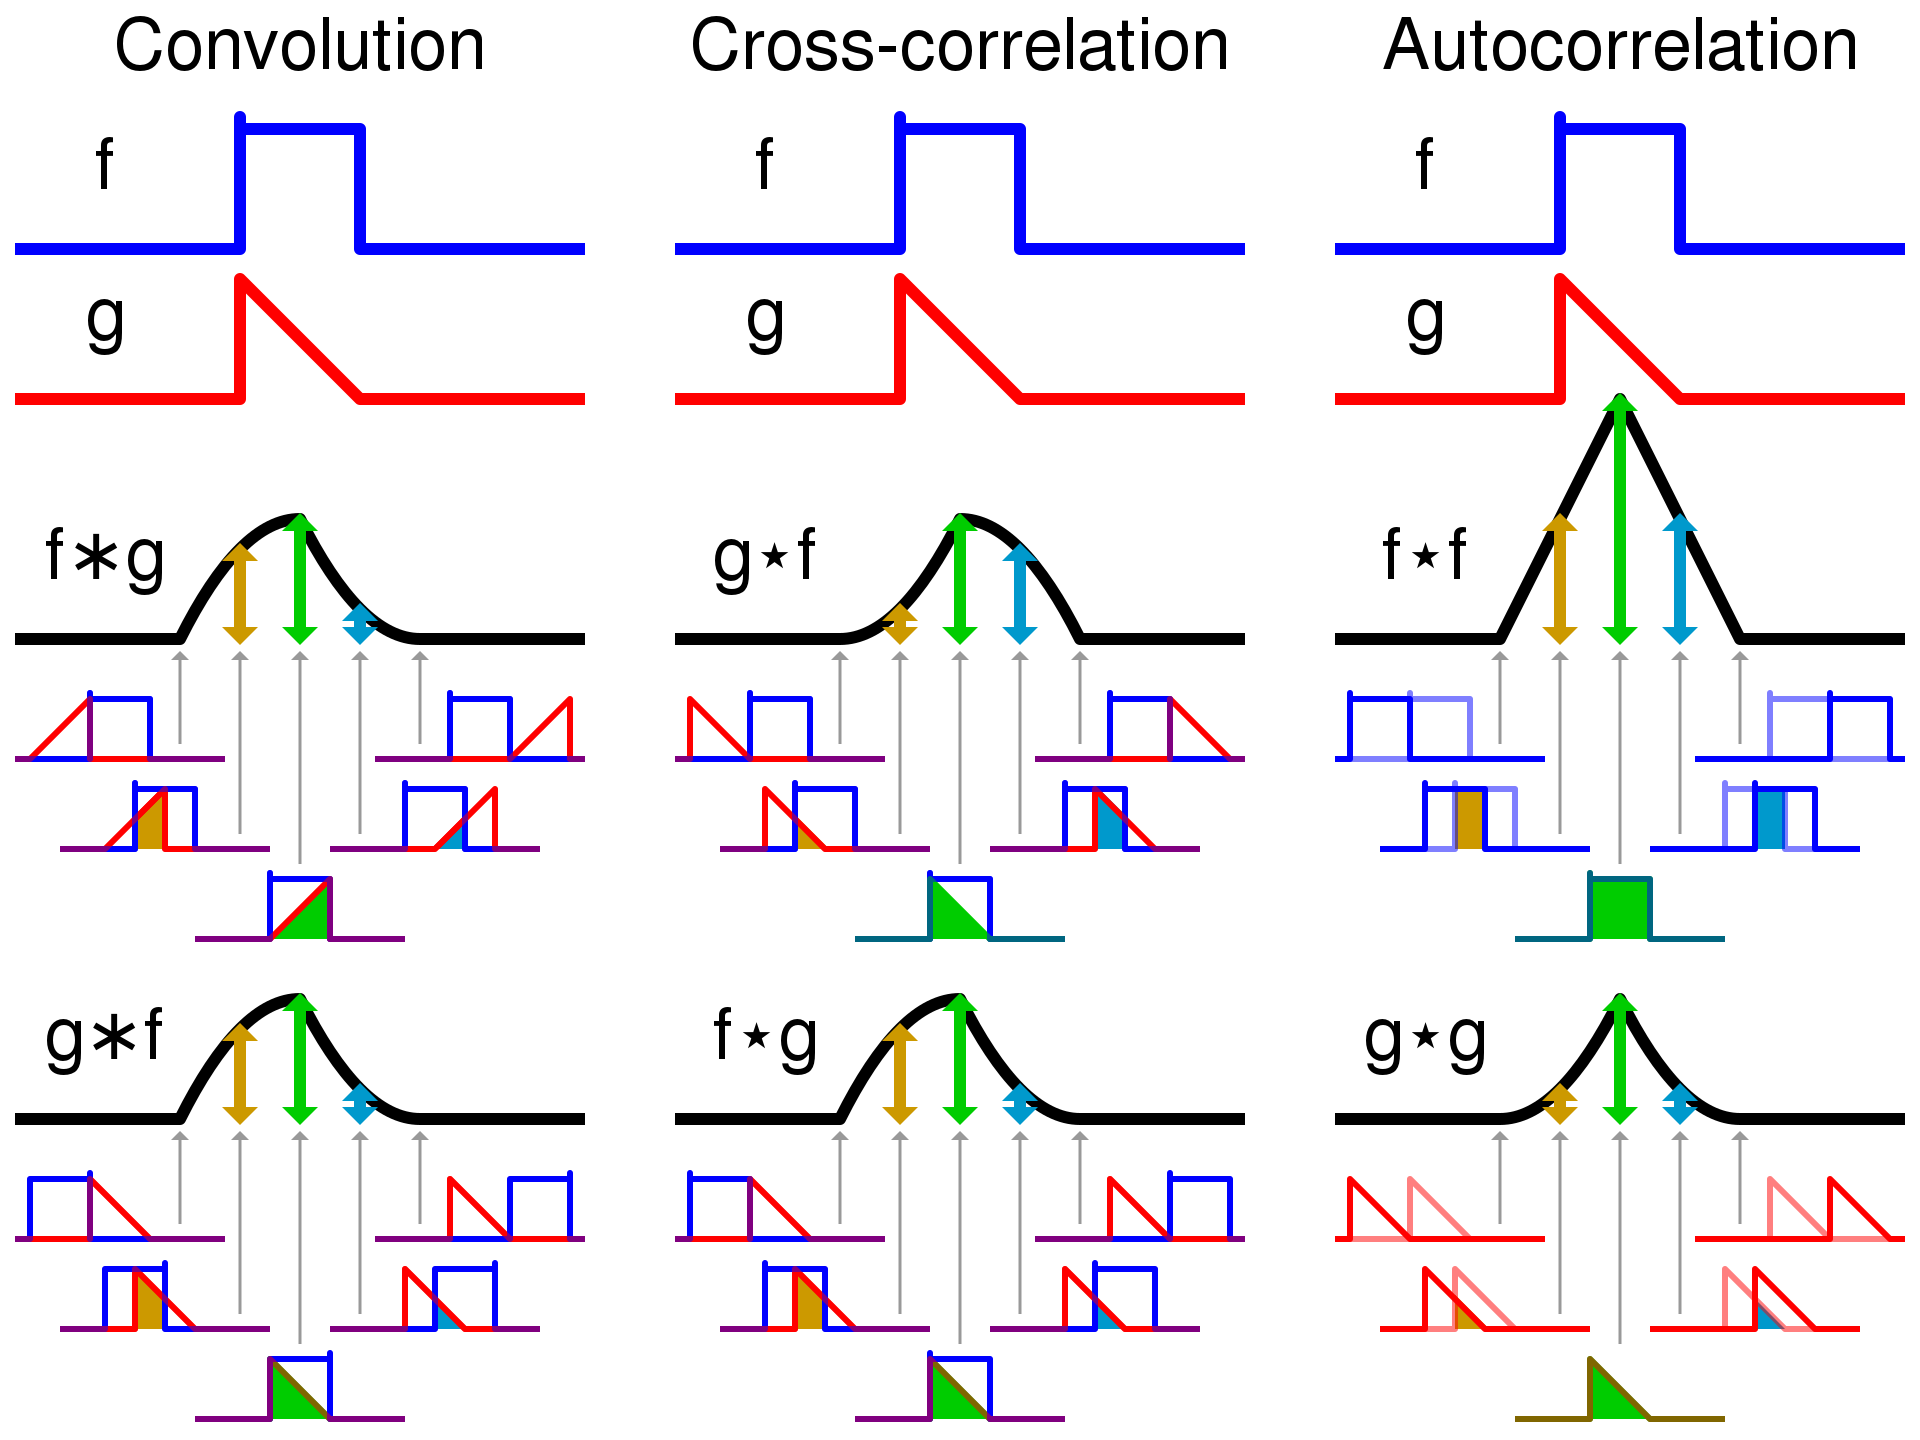
\includegraphics[height=2.5in]{Comparison_convolution_correlation.png}}
  \begin{tiny}
    By Cmglee, CC-SA 3.0,
    \url{https://commons.wikimedia.org/wiki/File:Comparison_convolution_correlation.svg}
  \end{tiny}
\end{frame}

\begin{frame}
  \frametitle{Autocorrelation is also a random variable!}

  \begin{itemize}
    \item Notice that, just as the power spectrum is a random
      variable, the autocorrelation is also a random variable.
    \item The autocorrelation is the average of $N$ consecutive
      products, thus
      \[
      E\left[r[n]\right] =
      E\left[\frac{1}{N}\sum_{m=0}^{N-1} x[m]x[m-n]\right]
      = E\left[x[m]x[m-n]\right]
      \]
      \ldots where the last form only makes sense if the signal is
      stationary (all samples identically distributed), so that
      $E\left[x[m]x[m-n]\right]$ doesn't depend on $m$.
    \item
      The expected autocorrelation is related to the covariance
      and the mean:
      \[
      E\left[r[n]\right] =\mbox{Cov}\left(x[m],x[m-n]\right)+E\left[x[m]\right]E\left[x[m-n]\right]
      \]
    \item
      If $x[n]$ is zero-mean, that means
      \[
      E\left[r[n]\right] =\mbox{Cov}\left(x[m],x[m-n]\right)
      \]
  \end{itemize}
\end{frame}
\begin{frame}
  \frametitle{Autocorrelation of white noise}
  If $x[n]$ is zero-mean white noise, then
  \[
  E\left[r[n]\right] =
  E\left[x[m]x[m-n]\right]= \begin{cases} \sigma^2 & n=0\\0 &\mbox{otherwise}\end{cases}
  \]
  We can write
  \[
  E\left[r[n]\right]=\sigma^2\delta[n]
  \]
\end{frame}

%%%%%%%%%%%%%%%%%%%%%%%%%%%%%%%%%%%%%%%%%%%%
\section[Summary]{Summary}
\setcounter{subsection}{1}

\begin{frame}
  \frametitle{Summary}
  \begin{itemize}
  \item Masking: a pure tone can be heard, in noise, if there is {\bf at least one}
    auditory filter through which $\frac{N_k+T_k}{N_k}>$ threshold.
  \item {\bf Parseval's Theorem:}
    \[
    \frac{1}{N}\sum_{n=0}^{N-1}x^2[n] = \frac{1}{N}\sum_{k=0}^{N-1}R[k]=
    \frac{1}{2\pi}\int_{-\pi}^{\pi}R(\omega)d\omega
    \]
  \item {\bf Wiener's Theorem:}
    \[
    R(\omega) \leftrightarrow r[n] = \frac{1}{N} x[n]\ast x[-n]
    \]
  \item The power spectrum and autocorrelation of noise are, themselves, random variables.
    For zero-mean white noise of length $N$, their expected values are
    \begin{align*}
      E\left[R[k]\right] &= \sigma^2\\
      E\left[r[n]\right] &= \sigma^2\delta[n]
    \end{align*}
  \end{itemize}
\end{frame}

\end{document}
